\documentclass[a4paper]{article}

\usepackage[T1]{fontenc}
\usepackage{textcomp}
\usepackage{amsmath, amssymb, amsthm}

\usepackage{setspace}
% figure support
\usepackage{import}
\usepackage{xifthen}
\usepackage{pdfpages}
\usepackage{transparent}

\title{Nuclear Lab Report}
\date{date}
\author{Jack Ruder and Tatum Bunnett}


\begin{document}

\doublespacing
\maketitle

\begin{figure}[htpb]
	\centering
	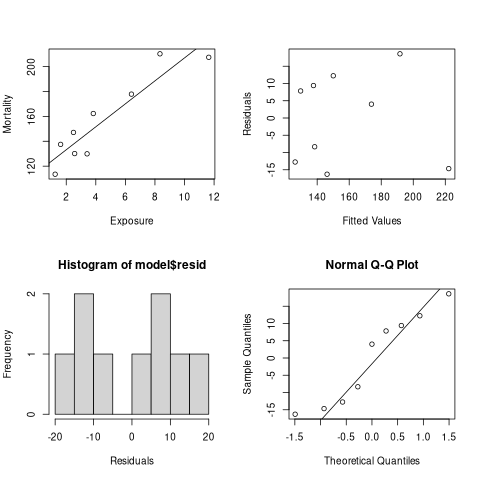
\includegraphics[width=\textwidth]{"../originalData.png"}
	\caption{Linear fit on non-transformed data}
	\label{fig:ogdat}
\end{figure}

\begin{figure}[htpb]
	\centering
	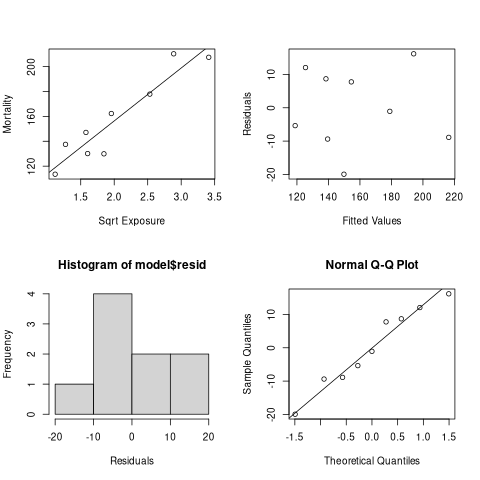
\includegraphics[width=\textwidth]{"../sqrtExposreXmortality.png"}
	\caption{Linear fit on transformed data}
	\label{fig:sqdat}
\end{figure}

\section{Model}
In examining the data, a linear model was fit to the original data, as seen in Figure \ref{fig:ogdat}. The basic fit showed that the data linear, though after experimentation, an even better fit was found using a square root transform on the Exposure data, seen in Figure \ref{fig:sqdat}. The fitted model is written as \begin{equation}M = 71.329 + 42.519 \cdot \sqrt{E}, \end{equation}
where \(M\) is the cancer mortality per 100000 man-years, and \(E\) is the index of exposure. Performing a t-test with this model gave a \(p\)-value for the slope of \(0.00017\), showing strong statistical significance of the model. We see an \(R^2\) of 0.88, confirming that Exposure and square-root Mortality are strongly correlated. 
However, this is not to say that there is no correlation between Exposure and Mortality, the fitted model without transforming Mortality had a p-value for the slope of 0.00033, and an \(R^2\) of 0.85. While the significance is not as strong, the linear model performs close enough to interperet meaning from its coefficients. The linear model is written as \begin{equation}M = 114.716 + 9.231 \cdot E.\end{equation}. Thus, for every unit index of exposure, we see that an additional 9 out of every 100000 deaths will occur. A confidence interval shows that with 95\% confidence 

\end{document}
